%!TEX root = elastic_3d_sbp.tex
\subsubsection{Iterative methods}\label{iterative_section}
In the proposed scheme (\ref{elastic_semi_c}), (\ref{fine_scheme}) and (\ref{continuous_sol})--(\ref{continuous_traction}), we need to solve a $3n^{2h}n^{2h}\times 3n^{2h}n^{2h}$ linear system at each time step twice for the continutiy of the traction force along the interface (\ref{traction_gamma_pre}) and (\ref{traction_gamma_corr}). Even though we can LU factorize the linear system before the time loop and reuse it at each time step, it is very expensive and memory inefficient to do LU factorization for a large problem. Besides, consider solving real problems which are usually in large scale, we want to perform the computation on many processors on a parallel distributed memory machine, but it is not clear how to calculate the LU factorization of a matrix on many processors. 

We have considered three iterative methods: the block Jacobian method, the conjugate gradient method, and the preconditioned conjugate gradient method. We note that the linear system arising from the interface conditions is indefinite. However, our experiment show that both the conjugate gradient method and the preconditioned conjugate gradient method converge. Except the following test that compares the three iterative methods, we always use the block Jacobian method to garantee that the whole scheme converges. 

For the problem proposed in Section \ref{manufactured_sol}, the structure of the coefficient matrix of the linear system (\ref{continuous_traction}) is shown in Figure \ref{Mass_matrix} which is determined by the interplation operator $\wt{\mathcal{P}}$ and restriction operator $\wt{\mathcal{R}}$. We choose the red circles in the purple circles in Figure \ref{Mass_matrix} to be the block Jacobian matrix in block Jacobian iterative method and pre-conditioning matrix in pre-conditioned conjugate gradient iterative method. The absolute error tolerance is set to be $1e-7$ for each iterative method.

\begin{table}[htbp]
	\begin{center}
		\begin{tabular}{|c|c c c|}
			\hline
			$h^c_k = 2h^f_k$   & ~~~~ CG ~~~~& Block Jacobian & Preconditioned CG  \\
			\hline
			$2\pi/24$ &37.78& 24.96& 4.01\\
			\hline
			$2\pi/48$ &38.61 & 25.38 & 2.87\\
			\hline 
			$2\pi/96$ &39.14 &25.43 & 2.55\\
			\hline
		\end{tabular}
	\end{center}
	\caption{condition number of matrices in conjugate gradient method, block Jacobian method, preconditioned conjugate gradient method}\label{condition_number}
\end{table} 
Table \ref{condition_number} shows the condition number of the original coefficient matrix, the block Jacobian matrix and the coefficient matrix after applying pre-conditioner respectively. We observe that the condition number for preconditioned conjugate gradient method is smallest which is consistent with the results for iteration number of different iterative methods : there is around $44$ iterations for conjugate gradient method, $13$ iterations for block Jacobian method and $9$ iterations for preconditioned conjugate method.

In comparison, we have also performed an LU factorization for the linear system when the mesh size $h^c = 2\pi/96$, and the computation takes 40.6 GB memory. In contrast, with the block Jacobian method, the peak memory usage is only 1.2 GB. For large-scale problems, the memory usage becomes infeasible for the LU factorization. 

\begin{figure}[H]
	\centering
	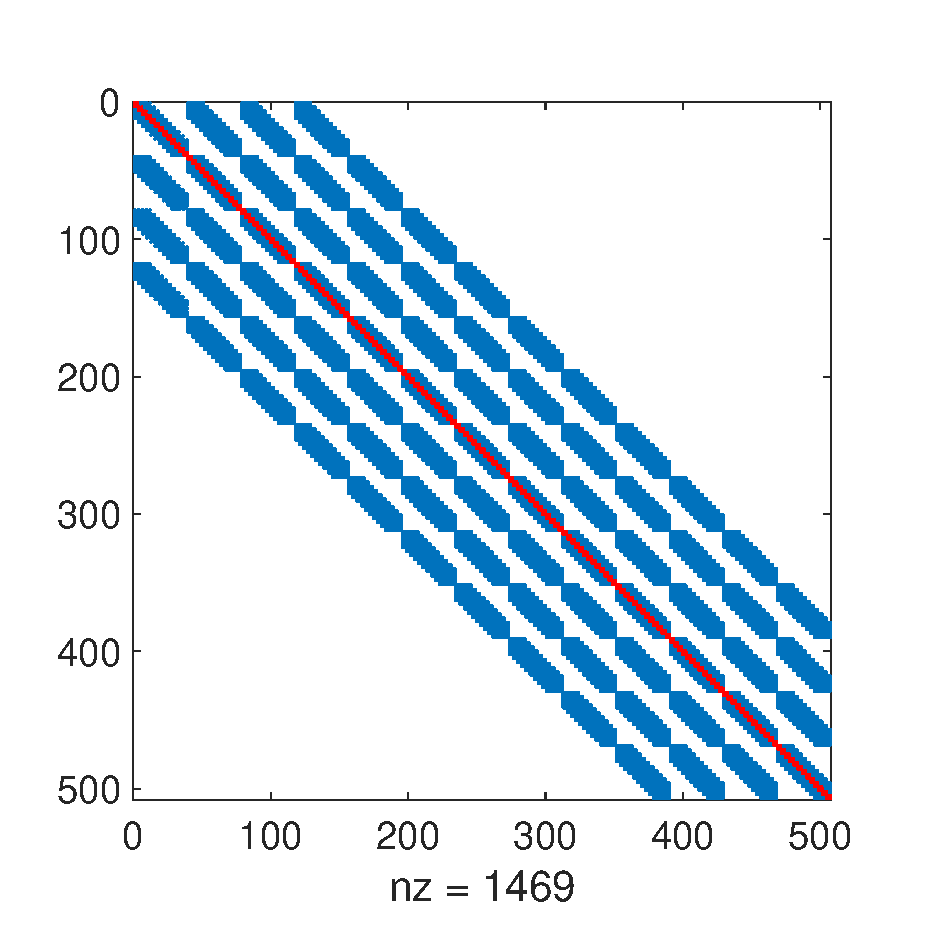
\includegraphics[width=0.45\textwidth,trim={1.2cm 1cm 1.4cm 1.2cm}, clip]{Mass_matrix.eps}
	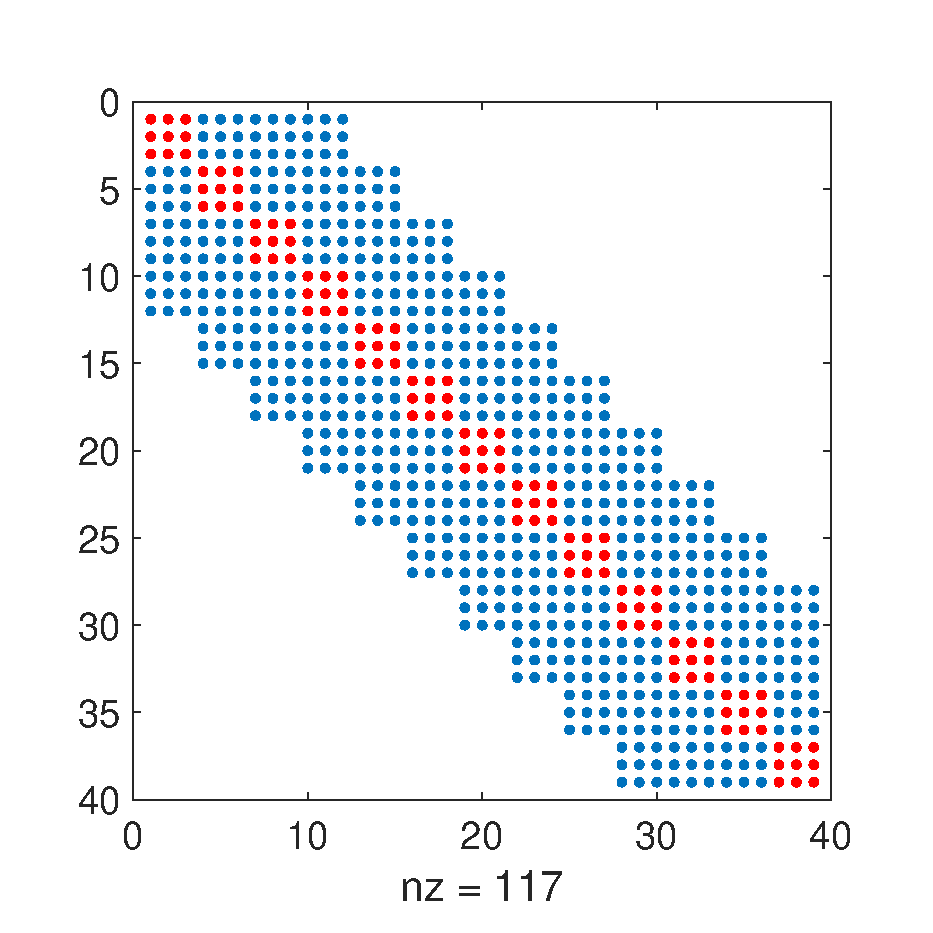
\includegraphics[width=0.45\textwidth,trim={1.2cm 1cm 1.4cm 1.2cm}, clip]{Mass_diagonal_matrix.eps}
	\caption{The left panel is the structure of the coefficient matrix of the linear system (\ref{continuous_traction}). The right panel is the zoom in structure for the repeated pattern on the left panel.}\label{Mass_matrix}
\end{figure}
